\documentclass[tikz,border=10pt]{standalone}
\usepackage{xcolor}
\usepackage{tikz}
\usetikzlibrary{arrows.meta, positioning, fit, backgrounds, calc}

% --- Anthropic-inspired color tokens ---
\definecolor{bgWarm}{HTML}{FAF8F3}
\definecolor{bgPanel}{HTML}{FFFDFC}
\definecolor{laneStroke}{HTML}{D7D0C5}
\definecolor{connectorStroke}{HTML}{9EA9B1}
\definecolor{inkText}{HTML}{31424B}
\definecolor{mutedText}{HTML}{66757E}

\definecolor{lavFill}{HTML}{E7E3FF}
\definecolor{lavStroke}{HTML}{8D86D8}
\definecolor{lavText}{HTML}{373457}
\definecolor{lavSubtext}{HTML}{5852A7}

\definecolor{mintFill}{HTML}{DDF4EC}
\definecolor{mintStroke}{HTML}{78B5A7}
\definecolor{mintText}{HTML}{294B45}
\definecolor{mintSubtext}{HTML}{3F8F7F}

\definecolor{tealFill}{HTML}{D9F0F2}
\definecolor{tealStroke}{HTML}{6CA9B0}
\definecolor{tealText}{HTML}{29464A}
\definecolor{tealSubtext}{HTML}{457E85}

\definecolor{creamFill}{HTML}{F4EEE3}
\definecolor{creamStroke}{HTML}{C1B39E}
\definecolor{creamText}{HTML}{4E4437}
\definecolor{creamSubtext}{HTML}{8E7A61}

\definecolor{amberFill}{HTML}{F8E7C9}
\definecolor{amberStroke}{HTML}{D6A86B}
\definecolor{amberText}{HTML}{57401C}
\definecolor{amberSubtext}{HTML}{A27431}

\definecolor{peachFill}{HTML}{F8E0D9}
\definecolor{peachStroke}{HTML}{CF8E81}
\definecolor{peachText}{HTML}{55342E}
\definecolor{peachSubtext}{HTML}{A66559}

\pagecolor{bgWarm}

\newcommand{\anthropicLabel}[4]{%
  \def\tmp{#4}%
  \ifx\tmp\empty
    {\sffamily\bfseries\small\textcolor{#1}{#3}}%
  \else
    \begin{tabular}{@{}c@{}}
      {\sffamily\bfseries\small\textcolor{#1}{#3}}\\[-1pt]
      {\sffamily\fontsize{8}{9}\selectfont\textcolor{#2}{#4}}
    \end{tabular}%
  \fi
}

\begin{document}

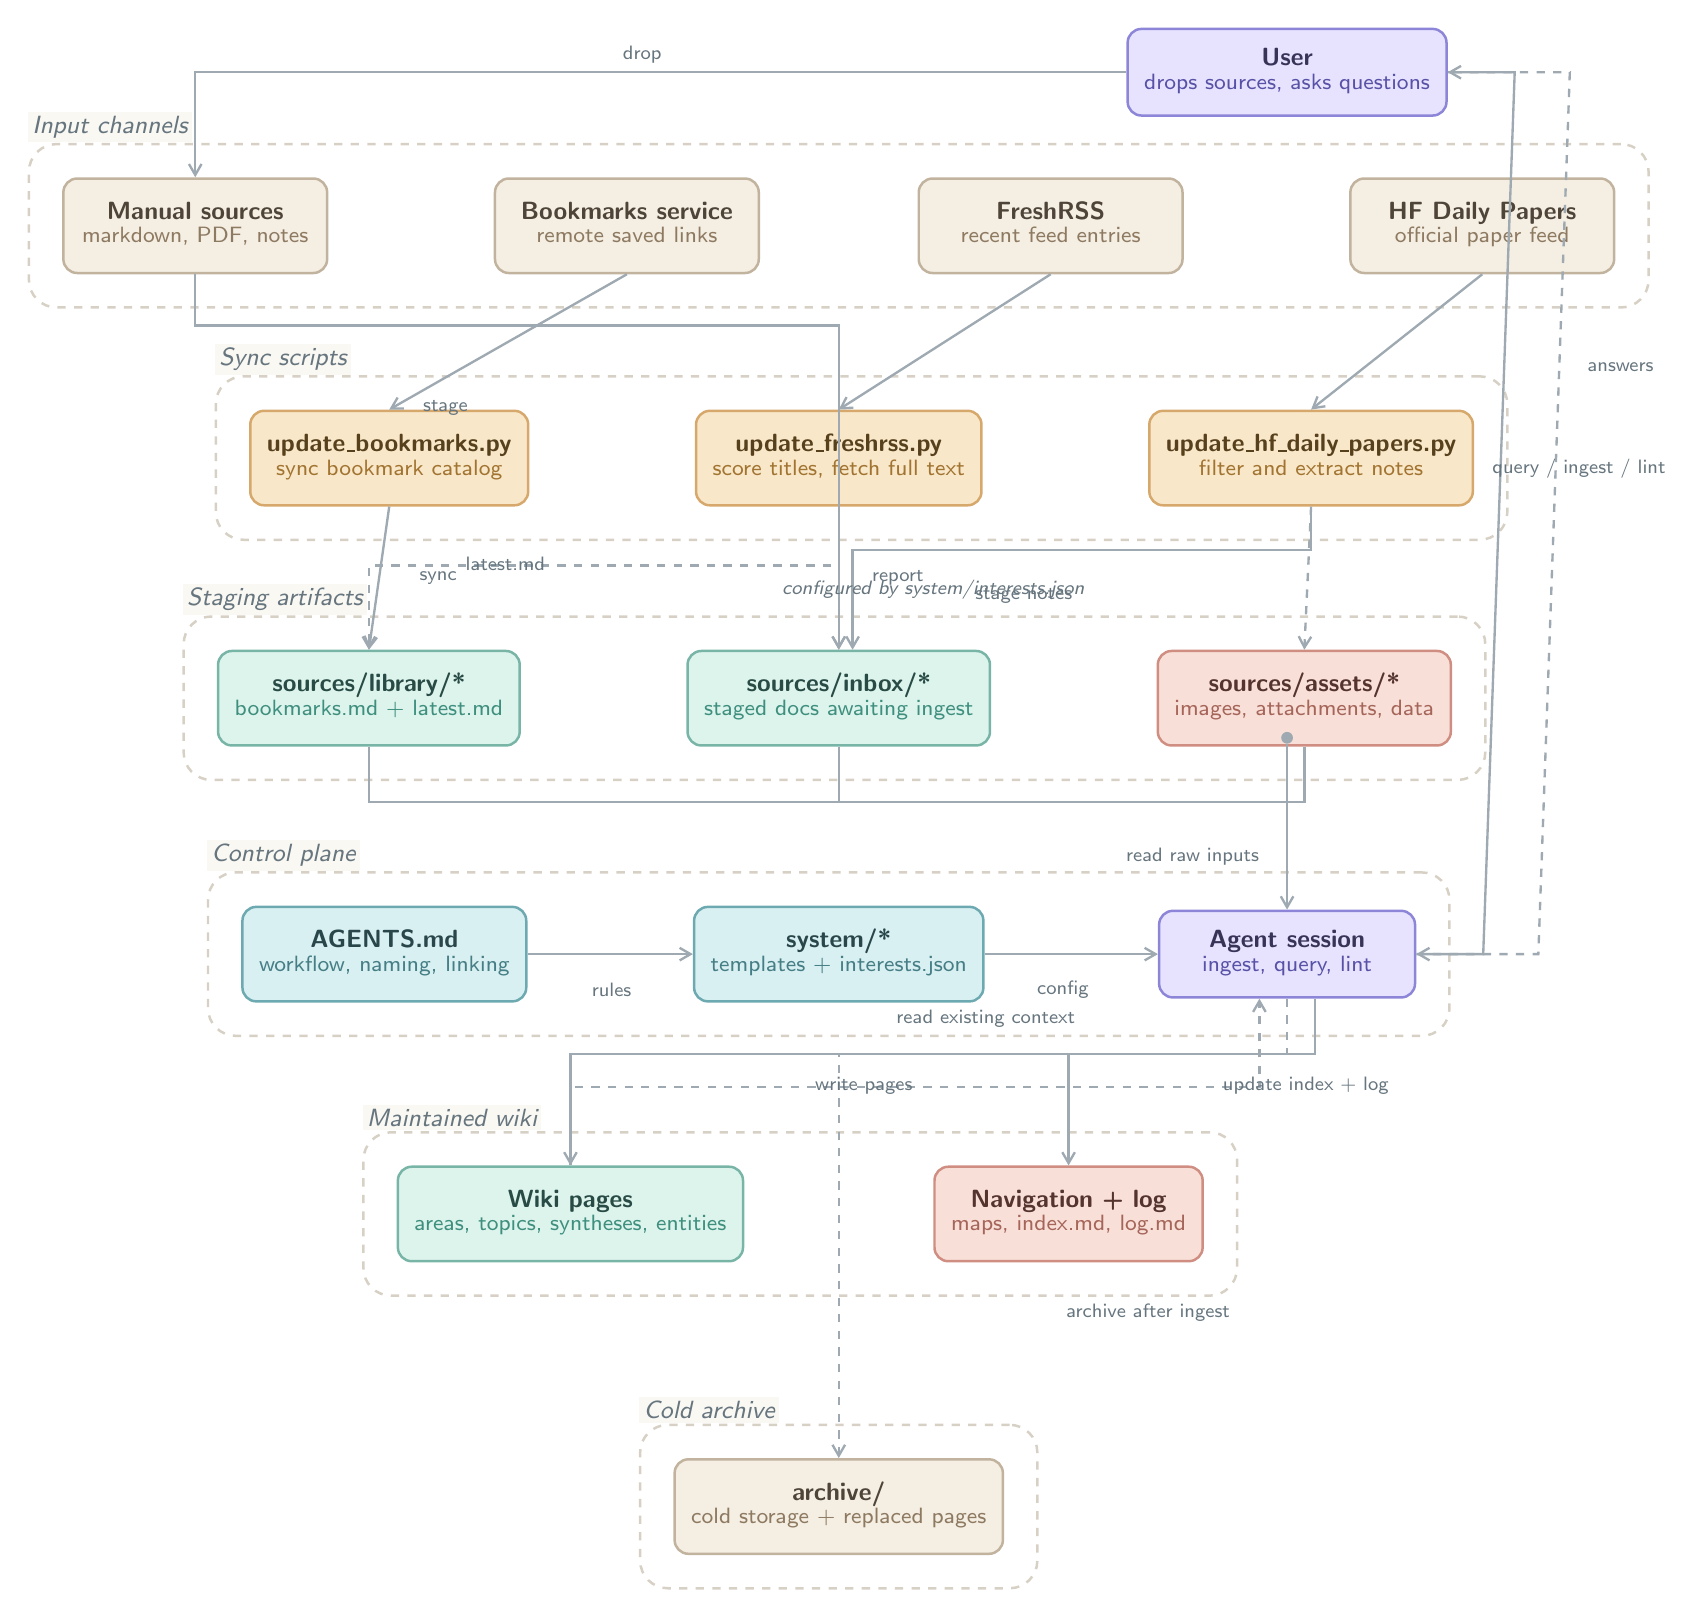
\begin{tikzpicture}[
    font=\sffamily\footnotesize,
    node distance=1.8cm and 2.0cm,
    anthropicEdge/.style={
        -{Straight Barb[angle=60:2pt 3]},
        draw=connectorStroke,
        line width=0.85pt
    },
    anthropicDashedEdge/.style={
        anthropicEdge,
        dashed
    },
    anthropicBus/.style={
        draw=connectorStroke,
        line width=0.85pt
    },
    anthropicCardNode/.style={
        rectangle,
        rounded corners=5pt,
        draw,
        line width=0.9pt,
        minimum width=3.35cm,
        minimum height=1.2cm,
        inner sep=6pt,
        align=center,
        fill=bgPanel
    },
    anthropicEventNode/.style={
        anthropicCardNode,
        minimum width=3.25cm,
        minimum height=1.1cm
    },
    anthropicGroup/.style={
        rectangle,
        rounded corners=10pt,
        draw=laneStroke,
        dashed,
        line width=0.9pt,
        inner sep=12pt,
        fill opacity=0
    },
    anthropicGroupTitle/.style={
        font=\sffamily\itshape\small,
        text=mutedText,
        fill=bgWarm,
        inner sep=1.5pt
    },
    edgeLabel/.style={
        font=\sffamily\scriptsize,
        text=mutedText,
        inner sep=1.5pt,
        fill=none,
        align=center
    }
]

    % ----------------------------------------------------------------
    % Layout: horizontal swimlanes stacked vertically, with the user
    % kept outside the lanes so interaction edges do not cut through
    % the source and sync cards.
    % ----------------------------------------------------------------

    % === Swimlane 1: Input channels ===
    \coordinate (inputCenter) at (0, 0);
    \node[anthropicCardNode, draw=creamStroke, fill=creamFill, left=1.0cm of inputCenter] (bookmarks)
        {\anthropicLabel{creamText}{creamSubtext}{Bookmarks service}{remote saved links}};
    \node[anthropicCardNode, draw=creamStroke, fill=creamFill, right=1.0cm of inputCenter] (freshrss)
        {\anthropicLabel{creamText}{creamSubtext}{FreshRSS}{recent feed entries}};
    \node[anthropicCardNode, draw=creamStroke, fill=creamFill, left=2.1cm of bookmarks] (manual)
        {\anthropicLabel{creamText}{creamSubtext}{Manual sources}{markdown, PDF, notes}};
    \node[anthropicCardNode, draw=creamStroke, fill=creamFill, right=2.1cm of freshrss] (papers)
        {\anthropicLabel{creamText}{creamSubtext}{HF Daily Papers}{official paper feed}};

    % === Swimlane 2: Sync scripts ===
    \coordinate[below=2.95cm of inputCenter] (syncCenter);
    \node[anthropicCardNode, draw=amberStroke, fill=amberFill] (rssscript) at (syncCenter)
        {\anthropicLabel{amberText}{amberSubtext}{update\_freshrss.py}{score titles, fetch full text}};
    \node[anthropicCardNode, draw=amberStroke, fill=amberFill, left=2.1cm of rssscript] (bookscript)
        {\anthropicLabel{amberText}{amberSubtext}{update\_bookmarks.py}{sync bookmark catalog}};
    \node[anthropicCardNode, draw=amberStroke, fill=amberFill, right=2.1cm of rssscript] (paperscript)
        {\anthropicLabel{amberText}{amberSubtext}{update\_hf\_daily\_papers.py}{filter and extract notes}};

    % === Swimlane 3: Staging artifacts ===
    \coordinate[below=3.05cm of syncCenter] (stageCenter);
    \node[anthropicCardNode, draw=mintStroke, fill=mintFill] (inbox) at (stageCenter)
        {\anthropicLabel{mintText}{mintSubtext}{sources/inbox/*}{staged docs awaiting ingest}};
    \node[anthropicCardNode, draw=mintStroke, fill=mintFill, left=2.1cm of inbox] (library)
        {\anthropicLabel{mintText}{mintSubtext}{sources/library/*}{bookmarks.md + latest.md}};
    \node[anthropicCardNode, draw=peachStroke, fill=peachFill, right=2.1cm of inbox] (assets)
        {\anthropicLabel{peachText}{peachSubtext}{sources/assets/*}{images, attachments, data}};

    % === Swimlane 4: Control plane ===
    \coordinate[below=3.25cm of stageCenter] (controlCenter);
    \node[anthropicCardNode, draw=tealStroke, fill=tealFill] (system) at (controlCenter)
        {\anthropicLabel{tealText}{tealSubtext}{system/*}{templates + interests.json}};
    \node[anthropicCardNode, draw=tealStroke, fill=tealFill, left=2.1cm of system] (agents)
        {\anthropicLabel{tealText}{tealSubtext}{AGENTS.md}{workflow, naming, linking}};
    \node[anthropicEventNode, draw=lavStroke, fill=lavFill, right=2.2cm of system] (agent)
        {\anthropicLabel{lavText}{lavSubtext}{Agent session}{ingest, query, lint}};
    \node[anthropicEventNode, draw=lavStroke, fill=lavFill] (user)
        at ($(agent |- inputCenter)+(0,1.95cm)$)
        {\anthropicLabel{lavText}{lavSubtext}{User}{drops sources, asks questions}};

    % === Swimlane 5: Maintained wiki ===
    \coordinate[below=3.3cm of controlCenter] (wikiCenter);
    \node[anthropicCardNode, draw=mintStroke, fill=mintFill, left=1.2cm of wikiCenter] (pages)
        {\anthropicLabel{mintText}{mintSubtext}{Wiki pages}{areas, topics, syntheses, entities}};
    \node[anthropicCardNode, draw=peachStroke, fill=peachFill, right=1.2cm of wikiCenter] (nav)
        {\anthropicLabel{peachText}{peachSubtext}{Navigation + log}{maps, index.md, log.md}};

    % === Swimlane 6: Cold archive ===
    \node[anthropicCardNode, draw=creamStroke, fill=creamFill, below=3.1cm of wikiCenter] (archive)
        {\anthropicLabel{creamText}{creamSubtext}{archive/}{cold storage + replaced pages}};

    % ================================================================
    %  EDGES — laid out after node placement, using orthogonal routing
    % ================================================================

    % Input and staging
    \coordinate (userDropTurn) at ($(manual.north)+(0,0.8cm)$);
    \coordinate (userDropCorner) at (userDropTurn |- user.west);
    \draw[anthropicEdge] (user.west) -- (userDropCorner) -- (userDropTurn) -- (manual.north);
    \draw[anthropicEdge] (manual.south) -- ++(0, -0.65) -| (inbox.north);
    \draw[anthropicEdge] (bookmarks.south) -- (bookscript.north);
    \draw[anthropicEdge] (freshrss.south) -- (rssscript.north);
    \draw[anthropicEdge] (papers.south) -- (paperscript.north);

    % Sync scripts to artifacts
    \draw[anthropicEdge] (bookscript.south) -- (library.north);
    \draw[anthropicEdge] (rssscript.south) -- (inbox.north);
    \draw[anthropicDashedEdge] (rssscript.south) -- ++(0, -0.75) -| (library.north);
    \draw[anthropicEdge] (paperscript.south) -- ++(0, -0.55) -| ([xshift=5pt]inbox.north);
    \draw[anthropicDashedEdge] (paperscript.south) -- (assets.north);

    % Staging bus into agent session
    \node[circle, fill=connectorStroke, inner sep=1.5pt, above=2.1cm of agent] (readBus) {};
    \draw[anthropicBus] (library.south) -- ++(0, -0.7) -| (readBus);
    \draw[anthropicBus] (inbox.south)   -- ++(0, -0.7) -| (readBus);
    \draw[anthropicBus] (assets.south)  -- ++(0, -0.7) -| (readBus);
    \draw[anthropicEdge] (readBus) -- (agent.north);

    % Control plane and invocation
    \coordinate (queryRailTop) at ([xshift=0.85cm]user.east);
    \coordinate (queryRailBottom) at ([xshift=0.85cm]agent.east);
    \coordinate (answerRailTop) at ([xshift=1.55cm]user.east);
    \coordinate (answerRailBottom) at ([xshift=1.55cm]agent.east);
    \draw[anthropicEdge] (agents.east) -- (system.west);
    \draw[anthropicEdge] (system.east) -- (agent.west);
    \draw[anthropicEdge] (user.east) -- (queryRailTop) -- (queryRailBottom) -- (agent.east);
    \draw[anthropicDashedEdge] (agent.east) -- (answerRailBottom) -- (answerRailTop) -- (user.east);

    % Wiki read/write loop and archive
    \coordinate (contextTurn) at ($(pages.north)+(0,1.0cm)$);
    \coordinate (agentReadPort) at ([xshift=-10pt]agent.south);
    \coordinate (agentWritePort) at ([xshift=10pt]agent.south);
    \draw[anthropicDashedEdge] (pages.north) -- (contextTurn) -| (agentReadPort);
    \draw[anthropicEdge] (agentWritePort) -- ++(0, -0.7) -| (pages.north);
    \draw[anthropicEdge] (agentWritePort) -- ++(0, -0.7) -| (nav.north);
    \draw[anthropicDashedEdge] (agent.south) -- ++(0, -0.7) -| (archive.north);

    % Annotation
    \node[font=\sffamily\scriptsize\itshape, text=mutedText, align=center]
        at ($(rssscript.south)+(1.2,-1.05)$) {configured by system/interests.json};

    % Transparent edge labels
    \node[edgeLabel] at ($(user.west)!0.52!(userDropCorner)+(0,0.22)$) {drop};
    \node[edgeLabel] at ($(manual.south)!0.45!(inbox.north)+(-0.5,0.45)$) {stage};
    \node[edgeLabel] at ($(bookscript)!0.5!(library)+(0.75,0)$) {sync};
    \node[edgeLabel] at ($(rssscript)!0.5!(inbox)+(0.75,0)$) {report};
    \node[edgeLabel] at ($(rssscript.south)!0.5!(library.north)+(-1.25,0.18)$) {latest.md};
    \node[edgeLabel] at ($(paperscript.south)!0.5!(inbox.north)+(-0.65,-0.22)$) {stage notes};
    \node[edgeLabel] at ($(readBus)!0.55!(agent)+(-1.2,0)$) {read raw inputs};
    \node[edgeLabel] at ($(queryRailTop)!0.46!(queryRailBottom)+(1.0,0.12)$) {query / ingest / lint};
    \node[edgeLabel] at ($(answerRailTop)!0.34!(answerRailBottom)+(0.78,0.06)$) {answers};
    \node[edgeLabel] at ($(agents)!0.5!(system)+(0,-0.45)$) {rules};
    \node[edgeLabel] at ($(system)!0.5!(agent)+(0,-0.45)$) {config};
    \node[edgeLabel] at ($(contextTurn)!0.58!(agentReadPort)+(0.2,0.22)$) {read existing context};
    \node[edgeLabel] at ($(agentWritePort)!0.5!(pages.north)+(-1.0,-0.05)$) {write pages};
    \node[edgeLabel] at ($(agentWritePort)!0.5!(nav.north)+(1.45,-0.05)$) {update index + log};
    \node[edgeLabel] at ($(agent.south)!0.67!(archive.north)+(2.05,-0.08)$) {archive after ingest};

    % ================================================================
    %  GROUPS
    % ================================================================
    \begin{scope}[on background layer]
        \node[
            anthropicGroup,
            fit=(manual) (bookmarks) (freshrss) (papers),
            label={[anthropicGroupTitle, anchor=south west]north west:{Input channels}}
        ] {};
        \node[
            anthropicGroup,
            fit=(bookscript) (rssscript) (paperscript),
            label={[anthropicGroupTitle, anchor=south west]north west:{Sync scripts}}
        ] {};
        \node[
            anthropicGroup,
            fit=(library) (inbox) (assets),
            label={[anthropicGroupTitle, anchor=south west]north west:{Staging artifacts}}
        ] {};
        \node[
            anthropicGroup,
            fit=(agents) (system) (agent),
            label={[anthropicGroupTitle, anchor=south west]north west:{Control plane}}
        ] {};
        \node[
            anthropicGroup,
            fit=(pages) (nav),
            label={[anthropicGroupTitle, anchor=south west]north west:{Maintained wiki}}
        ] {};
        \node[
            anthropicGroup,
            fit=(archive),
            label={[anthropicGroupTitle, anchor=south west]north west:{Cold archive}}
        ] {};
    \end{scope}

\end{tikzpicture}

\end{document}
